\documentclass{article}[11pt]
\setlength{\topmargin}{-2cm}
\setlength{\textheight}{24cm}
\setlength{\oddsidemargin}{10mm}
\setlength{\evensidemargin}{10mm}
\setlength{\textwidth}{15cm}
\setlength{\parskip}{3mm}
\setlength{\parindent}{0mm}

\usepackage{epsfig}
\usepackage{comment}
\usepackage{graphics}
\usepackage{graphicx}

\newcommand{\Rfunction}[1]{{\texttt{#1}}}
\newcommand{\Robject}[1]{{\texttt{#1}}}
\newcommand{\Rpackage}[1]{{\textit{#1}}}

\begin{document}

\section{Introduction}\label{Sec:Intro}

\subsection{Background}\label{Ssec:Backg}

There are many ways to visualize multivariate data where more than
two or three dimensions are needed to view the data.  Several of these ideas
were discussed in a previous paper, titled ``Creating Linked, Interactive
Plots to Explore Multivariate Data'', so the focus in this paper will be one
particular method of visualizing multivariate data that is particularly useful
for exploratory data analysis.  This paper will discuss creating linked,
interactive views of linked data sets.  

First brief definitions of linked and interactive views will be given.  Linked
plots mean that if a point on one plot changes its appearance, such as it
becomes colored red, then the corresponding point on a second plot will also
change its appearance to the color red.  For points to be corresponding, the
data displayed in the points must come from the same entity.  As an example,
suppose that the data consisted of each of the 50 states' murder rate, assault
rate, rape rate and percent of population living in urban areas.  Then if
there were two scatterplots, one with murder rate versus assault rate and the
other with rape rate versus percent urban population, the points on each plot
that referred to the state of Montana would be corresponding points.

Interactivity is an idea that will be familiar from using the Internet.  For
example, clicking on a hyperlink on a web page results in a new web page
opening.  Another example is clicking on the login button after entering a
user name and password to view one's email.  Interactivity means that there is
a response to some user action.  

Creating interactive applications requires three
things: some user action or input, which will be referred to as an
event; a response to that action, which will be executed by a callback
function; and a method that connects the event to the callback
function, which will be referred to as the signal handler.  These
three steps are ordered as follows: an event occurs, the event causes a
signal to be emitted that is caught by the signal handler, and then
the signal handler calls the callback function, which results in the
response to the user action.  A flowchart of these steps is shown
below in Figure \ref{Fig:Event}.  In the example of clicking on a
hyperlink mentioned above, the event is the user clicking on the
hyperlink and the callback function causes a new web page to open.
The signal handler, which is the method that connects the event to the
callback function, is not noticed by the user.  

\begin{figure}[!h]
  \begin{center}    
    \scalebox{0.8}{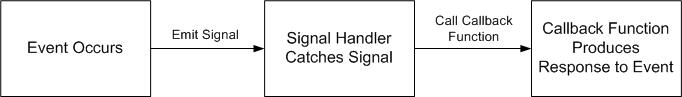
\includegraphics{Event.jpg}}
    \caption{ Flow Chart of the Response to an Event. }
    \label{Fig:Event}
  \end{center}
\end{figure}

This method of creating linked, interactive views of data is flexible for
exploring multivariate data because many different views can be created, such
as scatterplots, spreadsheets, and heatmaps, and then these views can be
linked.  Thus, users can decide which views best visually represent their
data.  Also, since the views are interactive, users can change the views while
looking at them to make the views more informative about the underlying data
structure.  This flexibility in linked, interactive views gives users a
powerful tool for visually exploring their data. 

\subsection{Design and Implementation of Linked, Interactive
  Views}\label{Ssec:Design} 

Focusing on linked, interactive views as a powerful visualization tool, the
next step is to determine how to design a software package that can implement
this method.  A popular design for creating linked views of data is the
model-view-controller (MVC) paradigm.  This design consists of three types
of objects: the controller, which defines what actions occur in response to
user input; the view, which consists of displays of the data; and the model,
which manages the data.  This paradigm is powerful because it decouples the
views from the model.  Thus, only one copy of the data needs to be stored and
then all views refer to this data set.  With all views based on the same data,
any changes to the data will be propagated to all views, which will give the
appearance of linked views.

To link the views to this one data set there is a subscribe/notify procedure
between the views and the model.  The views subscribe to a particular model
and the model must notify the views when a change occurs so that the views
will be updated.  This design allows multiple views of the model that are
linked, but are not aware of each other, as shown in Figure \ref{Fig:ExMVC}.

\begin{figure}[ht]
  \begin{center}
    \scalebox{0.7}{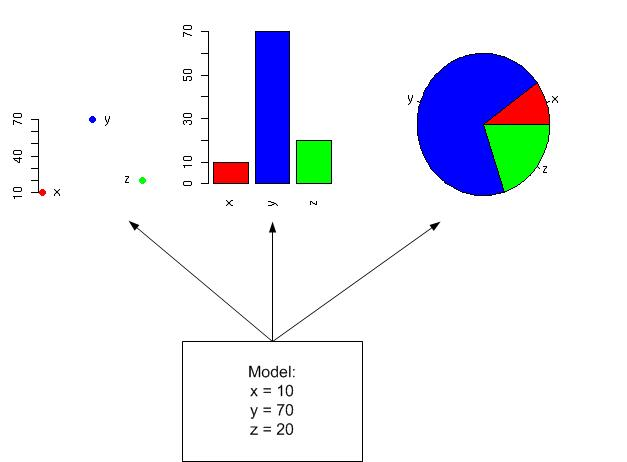
\includegraphics{ExMVC.jpg}}
    \caption{ A Model with its Views. }
    \label{Fig:ExMVC}
  \end{center}
\end{figure}

In the ``Creating Linked, Interactive Plots to Explore Multivariate Data''
paper, the creation of an R package called \Rpackage{iSPlot} was discussed.
The \Rpackage{iSPlot} package implemented the MVC design to satisfy three
goals: to create views that are linked, to create views that are interactive,
and to create a design that is extensible.  This package currently allows
users to generate linked, interactive scatterplots and spreadsheets of
two-dimensional data, such as data frames and matrices. 

\subsection{Limitations of the MVC Design}\label{Ssec:Limit}

The MVC design assumes that there is one data set that all views will
reference.  But what if the data consisted of more than one data set?  For
example, consider the data stored in a relational database.  Here there are
often multiple tables of data, where rows in different tables are linked
through a unique identifier called a key.  Although these tables of data
could be combined into one large table, there are several reasons not to do
this.  Keeping the data in separate tables reduces redundancy, particularly
when the rows are related by a one-to-many or a many-to-many relationship.
Also separate data tables lead to more maintainable data.  By storing only one
copy of each piece of information (in a row in one table), it is easier to
ensure that the data are correctly updated when a change occurs.  All other
tables that are connected with this information can then just reference this
row that has been updated.

Consider Figure \ref{Fig:DBTab} shown below.  Here the database consists of
three tables, Students, Classes, and StudentClasses.  The Students table has
four columns, StudentID (the key), FirstName, LastName, and Year.  The Classes
table has three columns, ClassID (the key), ClassName, and Department.  The
StudentClasses table has two columns, StudentID and ClassID.  This last table
relates which classes a student is taking and which students are in
each class.  In this example, the students can be taking more than one class
and each class can have more than one student.  So the relationship between
classes and students is many-to-many.  

%\clearpage

\begin{figure}[ht]
  \begin{center}
    \scalebox{0.5}{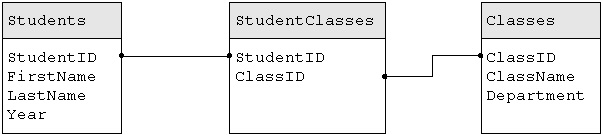
\includegraphics{databaseTables.jpg}}
    \caption{ Example of Relational Database Tables. }
    \label{Fig:DBTab}
  \end{center}
\end{figure}

Clearly, all of this data could be combined into one large
table, called CombinedStudentClass, as shown in Figure \ref{Fig:OneDBTab}.
The CombinedStudentClass table would have the following columns: StudentID,
FirstName, LastName, Year, ClassID, ClassName, and Department.  Now if a
student's last name changed, all instances of this student would need to be
changed in the new large table.  For example, if the student was taking four
classes, then this student would have four rows in the CombinedStudentClass
table and each row would need to change the value for the student's last name.
If instead only one record was kept per student, as shown in Figure
\ref{Fig:DBTab} above, then this process would be less error prone and would
require less memory to store the data. This example shows that there are
advantages to storing the data in separate structures. 

%\clearpage

\begin{figure}[ht]
  \begin{center}
    \scalebox{0.5}{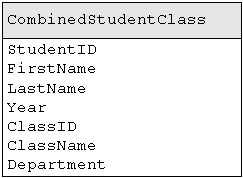
\includegraphics{oneDatabaseTable.jpg}}
    \caption{ Example of a Combined Table. }
    \label{Fig:OneDBTab}
  \end{center}
\end{figure}

In a relational database all of the data are stored in tables, but consider the
situation where there are multiple data sets that are of different data
structures.  For example, suppose that you have experimental microarray data,
which looks at gene expression levels.  This experimental data can be
stored as a two dimensional data structure, such as a matrix, where rows are
genes and columns are samples.  Linked to this
experimental data is meta data that gives information about the genes studied
in the microarray experiment.  This meta data may be a gene ontology
graph that gives the molecular functions of these genes.  These two data sets
(the experimental data and the meta data) are linked through the genes, but
they are different data structures.  The experimental data is a matrix and
the meta data is a graph.  

Now for the original MVC design, where one data set is expected, it is not
clear how to combine these two data sets into one data set.  The meta data
graph could be stored as a matrix, but a graph is a data structure that can be
well represented as an object with slots for nodes and edges, especially if
the graph is sparse.  As with the relational database tables, it seems
best in terms of data storage, alteration, and retrieval to keep the two data
sets separate.  Also, keeping the two data sets separate does not force a data
structure on the data that may not fit well.  

Currently, linked data sets are a common occurrence that can not be easily
visualized simultaneously.  Any time there is meta data linked to experimental
or study data there is a multiple data set situation where visually exploring
the data would be helpful to understand relationships between variables.  In
this paper, the design of software to create linked views based on multiple
linked data sets will be discussed.  The goals of this software will include
creating linked views of linked data sets, creating interactive
views where the response to an event can be changed, and creating
an extensible design that will allow future users to make additions.

\section{Extending the MVC Design}\label{Sec:Extend}

As discussed in Section \ref{Sec:Intro}, the MVC design expects one data set
with all views referencing this one data set.  However, several examples were
shown where multiple data sets are linked.  Since linking between multiple
data sets would be useful to visualize, the next step will be to determine how
the MVC design can be revised to account for multiple data sets.  

\subsection{One Large Data Set}\label{Ssec:OneDS}

One possibility for dealing with multiple data sets within the MVC design is to
combine the multiple data sets into one large data set.  With this new
combined data, the original MVC design will be appropriate for creating linked
views.  Thus, the strength of combining the data sets into one large data set
is that the MVC paradigm will already be appropriately set up to deal with the
one large data set. 

Unfortunately, as discussed in Section \ref{Ssec:Limit}, combining
multiple data sets into one large data set is not always appropriate or even
possible.  Even if the multiple data sets have the same data structure,
combining the data sets often results in redundant data and makes updating the
data more complicated.  In the situation where the data sets are not of the
same data structure, it may not be possible to combine the data sets into one
data structure that retains all of the original information.  Thus, another
way of linking views based on multiple data sets needs to be designed.

\subsection{Multiple MVC Objects}\label{Ssec:MMVC}

Because of the difficulty of combining multiple data sets, the MVC paradigm
will need to be altered to fit the data.  It has been mentioned that the MVC
design is intended to deal with one data set.  Now that we have several data
sets, why not have several MVC objects?  One MVC object to handle each data
set.  Thus, within each MVC object, one could create linked views of that
particular data set, which is the same as the original MVC design.  Then
between MVC objects a messaging system would need to be designed so that a
change in one data set would be sent to the other linked data sets.  

\small
\begin{tabular}[t]{ | l | r | r | }
  \hline
  State & Life Expectancy & Income \\ \hline
  Pennsylvania & 70.43 & 4449 \\ \hline
  California & 71.71 & 5114 \\ \hline
  Minnesota & 72.96 & 4675 \\ \hline
\end{tabular}
\hspace{10pt}
\begin{tabular}[t]{ | l | r | r | }
  \hline
  City & Precipitation & Temperature \\ \hline
  Philadelphia & 39.9 & 39 \\ \hline
  Pittsburgh & 36.2 & 37 \\ \hline
  Los Angeles & 14.0 & 68 \\ \hline
  San Francisco & 20.7 & 56 \\ \hline
  Sacramento & 17.2 & 55 \\ \hline
  Duluth & 30.2 & 18 \\ \hline
  Minneapolis St. Paul & 25.9 & 22 \\ \hline
\end{tabular}

\begin{table}[h]
  \begin{center}
    \begin{tabular}{ | r | r | }
      \hline
      State & City \\ \hline
      Pennsylvania & Philadelphia \\ \hline
      Pennsylvania & Pittsburgh \\ \hline
      California & Los Angeles \\ \hline
      California & San Francisco \\ \hline
      California & Sacramento \\ \hline
      Minnesota & Duluth \\ \hline
      Minnesota & Minneapolis St. Paul \\ \hline
    \end{tabular}
    \caption{State and City Values.}\label{Tab:CityState}
  \end{center}
\end{table}

\normalsize
As an example, suppose that one has two data sets: one with information at the
state level and one with information at the city level.  These tables are
shown in Table \ref{Tab:CityState}.  The State data includes Life Expectancy
(in years from 1970) and Income (per capita from 1974) data
while the City data includes Precipitation (in inches from 1975) and Average
High Temperature in January (in Fahrenheit from 2005)
data.  These two data sets are linked by the CityState table that links cities
with the states they reside in.  Now for these two data sets there would be
two MVC objects.  One MVC object for the State data and its views and one MVC
object for the City data and its views. 

\begin{figure}[ht]
  \begin{center}
    \scalebox{0.7}{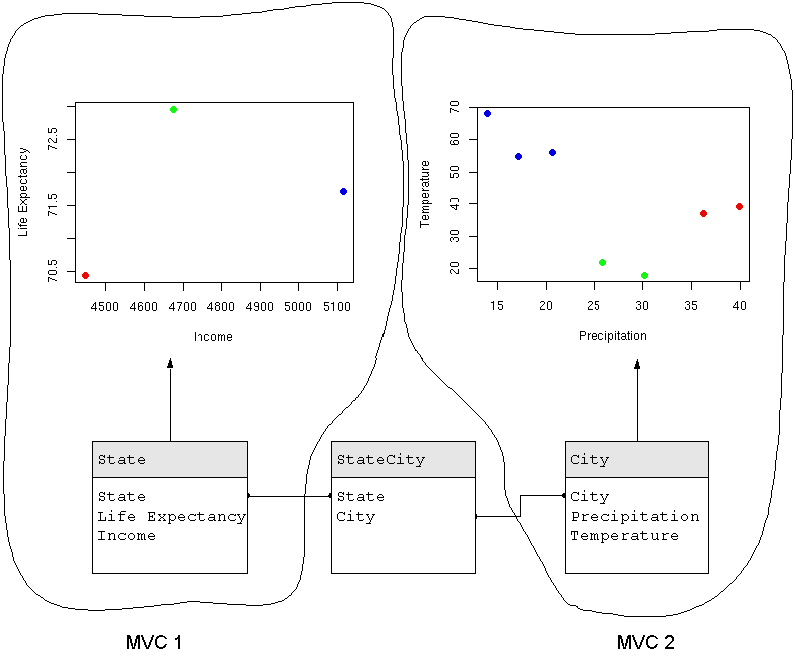
\includegraphics{MultipleMVC.jpg}}
    \caption{ Example of Two MVC Objects. }
    \label{Fig:MultMVC}
  \end{center}
\end{figure}

Figure \ref{Fig:MultMVC} shows one view for the State data and one view
for the City data.  You can see how the State and City data are linked based
on the coloring of the points in the plots.  The points referring to the state
of Pennsylvania are red, the points referring to California are blue, and the
points referring to Minnesota are green.  Even though there are two MVC
objects here, with one MVC object for each data set, it is still clear that
the views are linked through the data sets and that is shown in this example
through the coloring.

This solution uses the power and simplicity of the MVC design and expands it
to the multiple data set problem.  Now we can build on the original design,
which has been well tested, instead of starting a new design from scratch.
The strength of this multiple linked MVC design is that it uses MVC
components, which can be individually created and then linked.  Thus, these
components are reusable.  Also this multiple MVC design is structured to fit
with the linking seen in the multiple data sets.  Clearly, the design should
be built around the problem and multiple MVC objects with messaging between
the MVC objects fits the problem of creating linked views of multiple linked
data sets. 

Two parts of this design will need some special thought: creating an
appropriate messaging system between MVC objects and deciding how the MVC
objects will be related.  First, there are several questions that need to be
considered when creating the message system.  What information should be
passed between MVC objects in the messages?  Should there be a system to stop
messages from propagating between MVC objects?  How will the messages be
created and handled?  Second, there are also several questions with regard to
how the MVC objects will be related.  Should the MVC objects be related like
the tables in a relational database where the relationships are determined by
linked keys in different tables?  Should the MVC objects be linked through some
type of hierarchy, like a parent-child relationship where one MVC creates
another MVC and thus, the original MVC is the parent?  These decisions will be
based on the data that needs to be visualized and will be discussed in the
following sections as the design for multiple MVC objects is explained.

\section{Design Details of One MVC Object}\label{Sec:OneMVC}

\subsection{Overview}\label{SSec:OneOver}

Implementing a design to create linked, interactive views of multiple linked
data sets will be done in the R language in two packages, called
\Rpackage{MVCClass} and \Rpackage{iSNetwork}.  The \Rpackage{MVCClass} package
will implement the design of the MVC classes and methods.  The
\Rpackage{MVCClass} package will define the individual model, view, and
controller classes as well as the \Robject{MVC} class that binds the
individual model, view, and controller classes together into one unit.  The
package will also define the message classes that will allow the components to
communicate with each other.  The goal of separating these class definitions
and methods into one package is that they will be available for other R
packages that implement linked views of data, such as the \Rpackage{iSPlot}
and the \Rpackage{iSNetwork} packages.  

With the class definitions created in the \Rpackage{MVCClass} package, the
\Rpackage{iSNetwork} package will implement the graphical user interface
(GUI) so that users can load data, create views, and interact with the views
through a user interface with menus.  To create the GUI, \Rpackage{iSNetwork}
will use the R packages, \Rpackage{RGtk} and \Rpackage{gtkDevice}.
\Rpackage{RGtk} is an R package that allows one to interact with Gtk functions
from the R interface.  Gtk is an open-source X Window toolkit for creating
user interfaces.  The \Rpackage{gtkDevice} package creates a Gtk device by
turning a Gtk drawing area into a device that acts like an R device, but still
responds to events so that the view can be interactive.  For more information
about these packages, please see the paper, ``Creating Linked, Interactive
Plots to Explore Multivariate Data''. 

The next subsections will explain the class definitions and methods that
pertain to a single model-view-controller object.  Thus, the model classes,
the view classes, the controller, the \Robject{MVC} class (which binds the
model, view and controller classes together), and the message classes that pass
information between the three components in one MVC object will all be
discussed in the following subsections.  All of these definitions are
implemented in the \Rpackage{MVCClass} package.  Message class definitions
that pertain to communication between the MVC objects will be given in
Section \ref{Sec:MultMVC}.

\subsection{Model}\label{Ssec:OneModel}

The model class is responsible for storing and updating the data.  These two
functions are reflected in Figure \ref{Fig:Model}, which shows the inheritance
structure for the model classes.  Here the virtual class,
\Robject{gModel}, has the slots modelData, linkData, virtualData, and
modelName.  These four slots are common information that all models will
need.  The modelData slot is the data set for this model, the linkData slot is
a list of two functions, \Rfunction{linkToParent} and \Rfunction{linkToChild},
which link this model to its parent and child models, respectively (see Section
\ref{Ssec:MultLink}), the virtualData slot is data pertaining to the views
that needs to be stored with the model so that it can be shown in all views of
this model, and the modelName slot is the name of the model. 

\clearpage

\begin{figure}[ht]
  \begin{center}
    \scalebox{0.7}{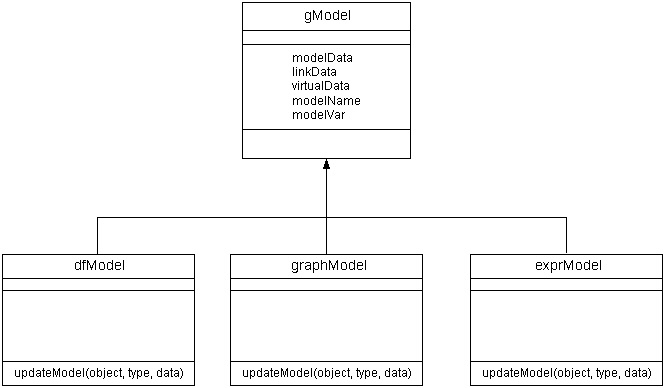
\includegraphics{ModelClass.jpg}}
    \caption{ Inheritance for Model Objects. }
    \label{Fig:Model}
  \end{center}
\end{figure}

For specific model classes, there are \Robject{dfModel}, \Robject{graphModel},
and \Robject{exprModel}.  The \Robject{dfModel} class represents a model where
the modelData has class data frame (or matrix), the \Robject{graphModel} class
represents a model where the modelData has class graph, and the
\Robject{exprModel} class represents a model where the modelData has class
exprSet. 

As mentioned previously, the model classes are also responsible for updating
the data and thus, you will notice that all three model classes have an
\Rfunction{updateModel} method.  This method is called whenever the data needs
to be updated in response to a user interacting with a view.  Thus, the
\Rfunction{updateModel} method is actually updating the virtualData slot
because it is this slot in the model classes that ensures that all views are
appropriately visually linked.

Although only three model classes are currently implemented, future users are
welcome to make additions to the model classes for new data structures they
would like to represent.  For example, a user may want to add a new model
class called \Robject{tsModel} to represent time series data.  

Note that the model classes must also notify views when the data has changed
so that the views can be updated.  The communication between a model and its
views will be discussed in Section \ref{Ssec:OneMess}. 

\subsection{Views}\label{Ssec:OneViews}

The view classes represent the visual depictions of the model.  All views will
need to store some common information and respond to certain events through
methods.  This consideration led to an object model where the different view
classes inherit from a view virtual class, called \Robject{genView}.  The
object model for the view classes is shown in Figure \ref{Fig:View}.

\begin{figure}[ht]
  \begin{center}
    \scalebox{0.7}{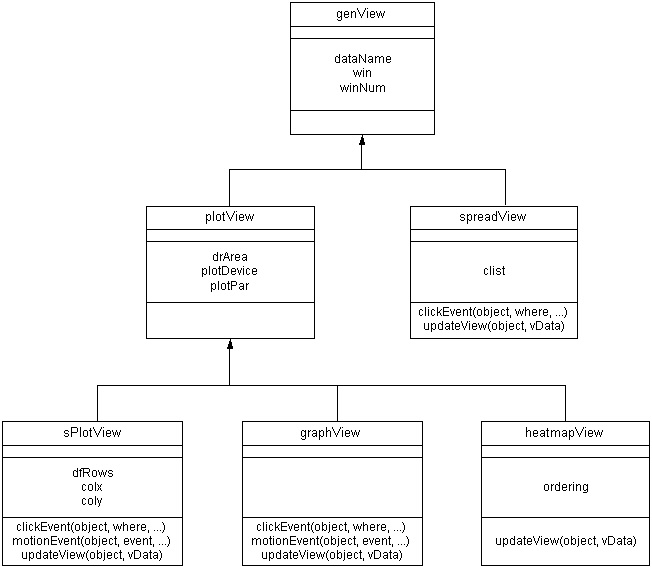
\includegraphics{ViewClass.jpg}}
    \caption{ Inheritance for View Objects. }
    \label{Fig:View}
  \end{center}
\end{figure}

The \Robject{genView} class has three slots, dataName, win, and winNum.
dataName is the name of the model that the view displays, win is the Gtk
window object that holds the view, and winNum is the number of the window so
that the window can be identified in the Window menu on the control window
(see Section \ref{Ssec:OneCont}).  All views will need to know these three
pieces of information so \Robject{genView} will bind the view classes
together. 

As for specific view classes, the \Robject{spreadView} class will represent a
spreadsheet view of the data.  This view will only make sense for models that
are a two dimensional data structure, such as a matrix or a data frame.  The
information needed for this view is stored in the slot, clist, which is the
Gtk spreadsheet object.

When creating a plot of a data set, there is a general class, called
\Robject{plotView}, that has the slots, plotDevice, plotPar, and drArea, which
store the device number of the plot, the plotting parameters, and the Gtk
drawing area object, respectively.  This class is not intended to have any
objects as it just represents a general plot.  The plot classes that can have
objects are the specific plot classes, \Robject{sPlotView},
\Robject{graphView}, and \Robject{heatmapView}, which inherit from the
\Robject{plotView} class.  

The \Robject{sPlotView} class represents a scatterplot view and it has the
extra slots, dfRows, colx, and coly, where dfRows are the row names from the
model that are shown in the plot, colx is the column name from the model that
is shown as the x variable in the plot, and coly is the column name from the
model that is shown as the y variable in the plot.  The \Robject{graphView}
class represents a graph plot view and it contains no extra slots besides
those in the \Robject{plotView} class.  The \Robject{heatmapView} represents a
heatmap view of the data and it contains the slot, ordering, which is a list
that is returned from the \Rfunction{heatmap} function to give information
about the dendrogram ordering.  Note that some of these views are only
applicable for certain model types. For example, the \Robject{graphView} class
will only make sense for a view of a graph object, which would be stored in the
\Robject{graphModel} class. 

Since all views are expected to be interactive, all
view classes have methods that correspond to user interaction, such as
\Rfunction{clickEvent}.  For \Robject{sPlotView}, the \Rfunction{clickEvent}
method is called when Gtk emits a signal that a mouse button has been pressed
and the \Rfunction{motionEvent} method is called when Gtk emits a signal that
the cursor has been moved over the view.  Both the \Rfunction{clickEvent} and
\Rfunction{motionEvent} methods for a \Robject{sPlotView} object will
determine which point on the plot was clicked or under the cursor,
respectively.  For \Robject{spreadView}, the \Rfunction{clickEvent} method is
called when Gtk emits a signal that a row in the spreadsheet has been selected
or unselected and the \Rfunction{clickEvent} will determine which row has
changed.  For \Robject{graphView}, the \Rfunction{clickEvent} method is called
when Gtk emits a signal that a mouse button has been pressed and the
\Rfunction{motionEvent} is called when Gtk emits a signal that the cursor has
been moved over the view.  Here, though, the \Rfunction{clickEvent} and
\Rfunction{motionEvent} methods will determine which node was clicked or under
the cursor, respectively.  Note that the \Robject{heatmapView} class has
neither a \Rfunction{clickEvent} or a \Rfunction{motionEvent} method because
currently, it is not possible to convert the user coordinates of where the
event occurred into some object on the view (such as the row and column
coordinates of the heatmap).  Thus, the \Robject{heatmapView} is the only view
that is not currently interactive.

As with the model classes, the view classes need an update method and thus, all
views have an \Rfunction{updateView} method.  This method must take the
information that a model has just been updated and appropriately update the
view to reflect that change.  Each method will depend on how the view
represents the data so for a \Robject{spreadView} object the
\Rfunction{updateView} may select or unselect a row on the spreadsheeet while
for a \Robject{sPlotView} object the \Rfunction{updateView} may change the
appearance of a point on the plot.

The inheritance structure of the view classes is intended to be extensible.
For instance, if users wanted to add a new plot view, say a density plot, they
could create a new view class that inherits from \Robject{plotView}, called
\Robject{dPlotView}.  This new class, \Robject{dPlotView}, would have slots
names dfRows and col to store which rows and which column, respectively, were
used to calculate the density shown in the view.

\subsection{Controller}\label{Ssec:OneCont}

The controller must perform several tasks, including storing information,
deciding how a view will respond to user interaction, and allowing users to
load data, to create views, and to quit the program.  These tasks can be
separated into two functions, where the first is that the controller needs to
be a storage location and the second is that the controller must be some type
of interactive interface that allows the user to determine the course of
actions.  

For the first function the controller will be an environment that is
stored in the controller slot of a MVC object, which will be discussed in more
detail in Section \ref{Ssec:OneMVC}.  This environment will store data
pertaining to state, such as information about appearance of the user interface
and the views.

For the second function the controller will be a GUI with menus to
allow the user to choose which action will occur next.  This aspect of the
controller, which is implemented in \Rpackage{iSNetwork}, is shown in the
Figure \ref{Fig:ContWin} and will be referred to as the control window. 

\begin{figure}[ht]
  \begin{center}
    \scalebox{0.5}{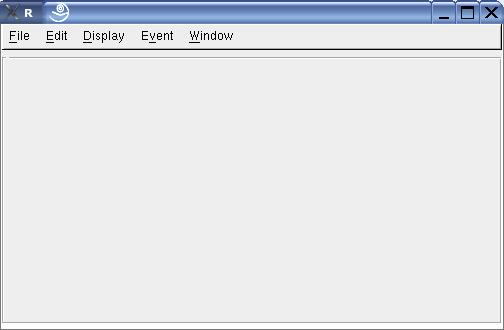
\includegraphics{ControlWindow.jpg}}
    \caption{ The Control Window. }
    \label{Fig:ContWin}
  \end{center}
\end{figure}

As shown in Figure \ref{Fig:ContWin}, the menus on the control window are
File, Edit, Display, Event, and Window.  These menus always appear on the
control window, but the menu items under each menu will change depending on
the type of model that is active.  Because the goal is to have multipled
linked MVC objects, there will be more than one MVC object and thus, more than
one model. However, the control window menus will only perform operations on
one MVC object at a time.  Thus, in the \Rpackage{iSNetwork} package there
will be the concept of the ``active'' MVC object, where the ``active'' MVC
object (and thus, the ``active'' model) means that operations performed
through the control window menus will affect that MVC object.  For example,
the Display menu allows users to create views of the active model, but only
certain views are appropriate for a type of model, as mentioned in Section
\ref{Ssec:OneViews}.  If the active model was a data frame model
(\Robject{dfModel}), then the views that the user could create would be a
scatterplot (\Robject{sPlotView}) and a spreadsheet (\Robject{spreadView}),
but a graph plot (\Robject{graphView}) would not make sense.  Thus, when the
model in the ``active'' MVC is of class \Robject{dfModel}, then the Display
menu will have menu items to create a scatterplot and a spreadsheet.

Because interacting with the views should be driven by the user,
the Event menu allows the user to determine what response will occur when
there is user interaction with a view.  For example, the user may initially
want a point on a plot to become colored when the left button is pressed and
the cursor is over that point.  Then the user may decide that the point
should be hidden when the left button is pressed and the cursor is over that
point.  The Event menu lets the user decide if anything will happen in
response to a left button click, a middle button click, a right button click,
and mouse movement.  More information will be given in Section
\ref{Ssec:OneEvent} about linking an event with a function so that user
interaction with a view is flexible enough to allow for multiple outcomes.

Because one of the goals of creating linked views based on multiple linked
data sets is to create a software package that is flexible and extensible,
users will be able to add menus and menu items to the control window.  As an
example if a future programmer wants to add a new type of view, such as a
histogram, then a new menu item for that view could be added to the Display
menu, as long as that view makes sense for the active MVC's model.  By
allowing users to change the controller, they can add new functionality that
is specific to their problem.  

\subsubsection{Linking Events to Functions}\label{Ssec:OneEvent}

Linking callback functions to events, such as a button click, a mouse movement
or a key press event, is what allows users to have an interactive
environment.  Then when an event happens something will occur in response
depending on the callback function linked to the event.  Now to create a
flexible environment we do not want a callback function that always does the
same thing when an event occurs.  For example, when a left button press event
occurs, we may sometimes want a point to be colored and at other times we may
want a point to be hidden.  To allow this flexibility, a class called
\Robject{gEventFun} was created.  By using this class, users will be able to
change the response to an event.  

The \Robject{gEventFun} class stores all of the information about a potential
callback function.  When a user wants to connect this callback function to an
event, this can be performed through the Event menu on the control window (see
Section \ref{Ssec:OneCont}).  The controller
environment in each MVC object will store which \Robject{gEventFun} object
(representing the callback function) is linked with each event.  Thus, the
user can decide the response for button clicks and mouse movements, and the
user can change these responses at any time through the control window.

\begin{figure}[ht]
  \begin{center}
    \scalebox{0.6}{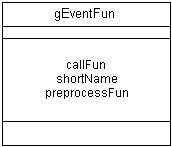
\includegraphics{EventClass.jpg}}
    \caption{ The gEventFun Class. }
    \label{Fig:EventFun}
  \end{center}
\end{figure}

As shown in Fig \ref{Fig:EventFun}, the slots in the \Robject{gEventFun} class
are callFun, shortName, and preprocessFun.  The callFun slot is the name of
the callback function, the shortName slot is a short description of the
function, and the preprocessFun slot is a character vector of all
preprocessing functions that must be called before the callback function.

The callback function that is stored in the callFun slot must take only one
parameter and the class of this parameter will depend on the model class in
the active MVC object.  For example, for a graph model, the
parameter will be of class \Robject{AgNode}, representing a node in the graph.
For a data frame model, the parameter will be of class character, representing
a row in the data frame.

The preprocessing functions that are stored in the preprocessFun slot will
take no parameters.  The purpose of the preprocessing functions is to set some
variables that the callback function will need.  Thus, not all callback
functions will need preprocessing functions and if no preprocessing functions
are needed, then this slot will be NULL.  If the callback function sets the
color of a node in a graph, then a preprocessing function is needed to
determine what color this will be.  So in this example, the preprocessing
function will open a color browser to allow the user to choose what the new
color will be.

\subsection{MVC}\label{Ssec:OneMVC}
 
The \Robject{MVC} class is the class that will bind the model, view, and
controller objects that refer to the same data set into one object.  Thus, the
creation of a MVC object occurs whenever a new data set is added.  A
MVC object can have one model and each model must be in one
MVC object so there is a one-to-one relationship between the
MVC and model objects.  Because of this relationship, the
MVC object and the model object are identified by the same name,
which is stored in the modelName slot of the model object. 

As shown in Figure \ref{Fig:MVCClass}, the \Robject{MVC} class has five slots
which are, model, viewList, controller, parentMVC, and childMVCList.  The
model slot stores the model object, the viewList slot is a list of the view
objects for this model, the controller slot is an environment that stores
information for this MVC, the parentMVC slot is the name of the parent model
(MVC), and the childMVCList slot is a list of the children models
(MVCs).  Note that model and MVC objects use the same name so the
parentMVC slot refers to both the name of the model and the name of the
MVC.  Similarly, for the childMVCList slot, the names in the list
refer to both the name of the model and the name of the MVC.

\begin{figure}[ht]
  \begin{center}
    \scalebox{0.6}{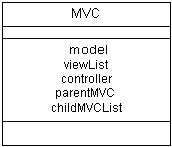
\includegraphics{MVCClass.jpg}}
    \caption{ The MVC Class. }
    \label{Fig:MVCClass}
  \end{center}
\end{figure}

Thus, the \Robject{MVC} class not only binds the model, view, and controller
objects together, but it also shows that the MVC objects are related
to each other through a parent-child (tree) hierarchy, as shown in Figure
\ref{Fig:Hier}.  In this picture, `model1' is the name of the original MVC
object (model) and from it, two MVC objects were created, `model2' and
`model3'. Then from `model2', three MVC objects were created, `model4',
`model5', and `model6'.  

\clearpage

\begin{figure}[ht]
  \begin{center}
    \scalebox{0.6}{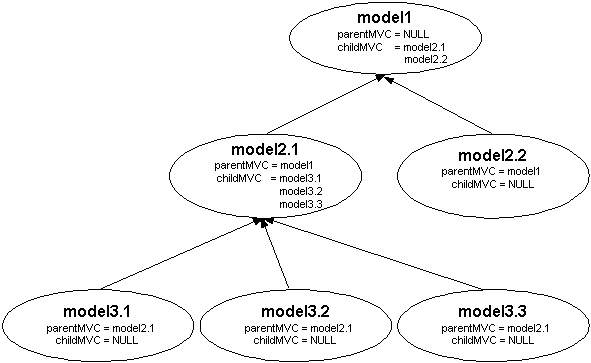
\includegraphics{Hierarchy2.jpg}}
    \caption{ The Parent-Child Relationship Between MVCs. }
    \label{Fig:Hier}
  \end{center}
\end{figure}

A MVC object can have at most one parent MVC, but it can have many child
MVCs.  The relationship between MVC objects shows that child MVC objects are
derived from the parent MVC object (i.e. the model in the child MVC is derived
from the model in the parent MVC).  An easy example of a child model derived
from a parent model is to start with a data frame as the parent model and then
take a subset of this data frame as the child model. 

\subsection{Messages}\label{Ssec:OneMess}

The message classes are intended to provide communication between different
components of the MVC design, such as when the model changes a message needs to
be sent to the views to let them know that they should be updated.  This
communication between the model, view and controller is crucial for the pieces
to work together and yet, still be independent of each other.  

The object model for the message classes was derived from the idea that all
messages must have certain methods in common, such as \Rfunction{initialize}
and \Rfunction{handleMessage}, because all messages must be created and
handled in some manner so that the message is read and acted upon.  Also,
since messages are sent when something has changed, either through addition,
alteration, or deletion, the message classes reflect only certain operations.
These common purposes for the messages allow the message object model to be
constructed, and this model is shown in Figure \ref{Fig:Mess}.

\begin{figure}[ht]
  \begin{center}
    \scalebox{0.6}{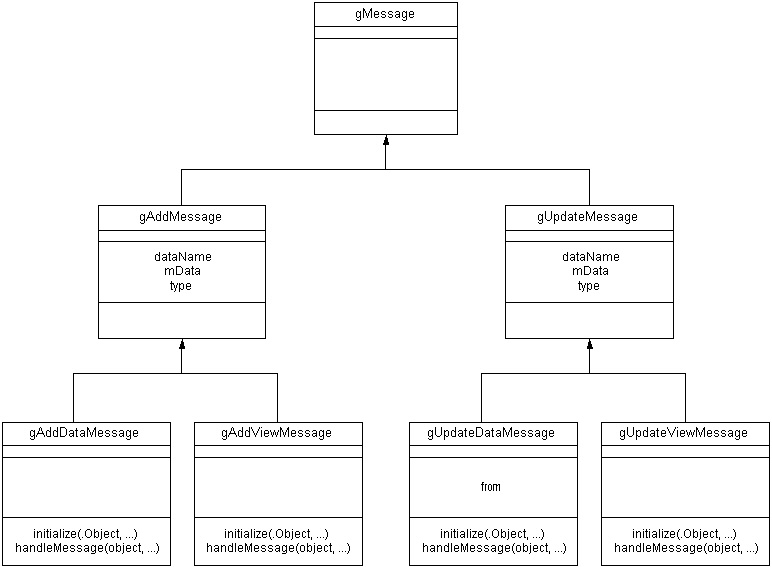
\includegraphics{MessageClass.jpg}}
    \caption{ Inheritance for Message Objects. }
    \label{Fig:Mess}
  \end{center}
\end{figure}

As with the view classes, the top message class, \Robject{gMessage}, is a
virtual class.  It contains no slots and its purpose is to bind the other
message classes together.

Currently, there are two types of messages for messaging within a model, view,
controller object: an add and an update message.  Both the add message,
\Robject{gAddMessage}, and the update message, \Robject{gUpdateMessage},
contain three slots, dataName, mData, and type.  dataName is the character
string that gives the name of the model, mData is a list of data needed to
perform the addition or alteration operation, and type is a character string
that gives the type of addition or alteration to perform.  Although
\Robject{gAddMessage} and \Robject{gUpdateMessage} are not virtual classes, it
is not intended to create objects of these classes.

Since adding a view requires different information and methods from adding a
model (and similarly with updating views versus models), it makes sense to
have two separate message classes for these operations.  Thus, when messages
are sent between components, they are from one of the following classes:
\Robject{gAddDataMessage}, \Robject{gAddViewMessage},
\Robject{gUpdateDataMessage}, and \Robject{gUpdateViewMessage}.  As shown in
Figure \ref{Fig:Mess}, the \Robject{gAddDataMessage} and
\Robject{gAddViewMessage} classes inherit from the \Robject{gAddMessage}
class, and the \Robject{gUpdateDataMessage} and \Robject{gUpdateViewMessage}
classes inherit from the \Robject{gUpdateMessage} class. 

The \Robject{gAddDataMessage} class represents a message to add a model and a
MVC object because whenever a model is added, a MVC object is also added that
contains this model.  The \Robject{gAddViewMessage} class represents a message
to create a view.  This message can only be used after a model has been
added.  

The \Robject{gUpdateDataMessage} class represents a message to update
a model.  This message is crucial for linking because it is responsible for
ensuring that once a model has been updated this information must propagate to
any views of the model and this information must also be passed along to any
other MVC object that is related to this model.  Because this information gets
passed to other MVC objects, which will be discussed further in Section
\ref{Sec:MultMVC}, this message also has one new slot, from, in addition to
the slots it inherits from \Robject{gUpdateMessage}.  The from slot is the
name of the model that the update data message came from.  This slot is
necessary because the update data message can come from one of two sources:
one the message can occur because of user interaction with a view
of this model or the message may occur because a different model that is
linked to this model has been updated.  So the update data message may come
from within this MVC object or it may come from a different MVC object that
has changed its model and is related to this MVC object.  
Information on passing messages between MVC
objects will be given in Section \ref{Sec:MultMVC}.  Finally, the
\Robject{gUpdateViewMessage} class represents a message to update a view.
This message will be created and handled whenever the model is updated so that
the views accurately reflect the model.

All four classes, \Robject{gAddDataMessage}, \Robject{gAddViewMessage},
\Robject{gUpdateDataMessage}, and \Robject{gUpdateViewMessage}, have
\Rfunction{initialize} and \Rfunction{handleMessage} methods, which perform
the following tasks:

\begin{list}{}{\setlength{\leftmargin}{0.5in}
               \setlength{\itemsep}{0in}}
  \item \Rfunction{initialize} is used to properly fill the slots of the
object when it is created.  
  \item \Rfunction{handleMessage} is necessary to
process the message.  Since a message is a form of communication
between two components, once it is created it must be sent to the
proper recipient and action must be taken in response to its
information, which is the purpose of the \Rfunction{handleMessage} method.
\end{list}

As with the inheritance structures seen in previous sections, the message
inheritance structure is designed to allow for extensibility.  For example, a
user could create a \Robject{gUpdateControlMessage} class that inherited from
the \Robject{gUpdateMessage} class.  This new class,
\Robject{gUpdateControlMessage}, could convey information that told the
control window to be updated in response to a change in the active MVC.
Recall from Section \ref{Ssec:OneCont} that the active MVC is the MVC object
that the menus on the control window refer to so any of the operations chosen
from the control window menus will be applied to this MVC object (the active
MVC).  The goal for the message classes is that the design is flexible enough
to allow a user to make additions or changes.

\section{Details of Multiple MVCs}\label{Sec:MultMVC}

Up until now we have skirted around the fact that multiple MVC objects are
being used in this design for linking views of multiple linked data sets.
Each MVC object will represent one model and its views.  Now for the views of
different data sets to be linked, they must link through the data sets so this
linking information must be stored somewhere.  Also, there must be
message classes to pass information between MVC objects.

As mentioned in Section \ref{Ssec:OneMVC}, the \Robject{MVC} class has slots
for how the current MVC relates to other MVC objects and these slots are
parentMVC and childMVCList.  These slots show that MVC objects are related
through a tree hierarchy where a child model is derived from its parent
model.  Consider Figure \ref{Fig:SmallHier} shown below.  If firstMVC's model
changes, then this information first gets passed to secondMVC, which may make
changes to its model based on this information.  Then secondMVC passes this
information to thirdMVC based on the changes secondMVC made to its model.
Thus, information passing between firstMVC and thirdMVC only occurs through
secondMVC.  So messages can only be sent from parent MVC to child MVC or from
child MVC to parent MVC.

\begin{figure}[ht]
  \begin{center}
    \scalebox{0.6}{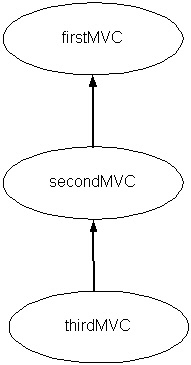
\includegraphics{SmallHierarchy.jpg}}
    \caption{ Multiple MVC Objects and Their Relationships. }
    \label{Fig:SmallHier}
  \end{center}
\end{figure}

Next we will consider how the data sets will be linked (and thus, how MVC
objects are linked) followed by how messages will be passed between these
linked MVC objects. 

\subsection{Linking Data Sets}\label{Ssec:MultLink}

For messages to pass between MVC objects, there must be a function or a place
that converts information from one MVC into useful information for a different
MVC object.  Thus, there needs to be some way to determine how data from one
MVC object relates to data in a different MVC object.  This conversion is done
by two functions that are stored in the linkData slot of the model objects.
The linkData slot is a list with two elements: a \Rfunction{linkToParent}
function and a \Rfunction{linkToChild} function.  

When a child MVC is created from an existing MVC, the child model's linkData
slot will be filled with the two functions, \Rfunction{linkToParent} and
\Rfunction{linkToChild}.  When the model in the child MVC is updated, the
\Rfunction{linkToParent} function in the linkData slot will be used to convert
the child model's data change into useful information for the parent model.  

Now suppose that the parent model changed instead.  This information
needs to be passed to the child model.  However, a parent can have multiple
child MVC objects so which \Rfunction{linkToChild} function should be used?
Here, when a parent is updated and needs to pass information to its children,
the \Rfunction{linkToChild} function is stored with each child MVC because a
parent MVC may have multiple child MVC objects that all need to process this
information in a different way.  Thus, when a child MVC object is created and
its model's linkData slot is filled, the \Rfunction{linkToParent} function
will convert information from this child model into useful information for its
parent MVC and the \Rfunction{linkToChild} function will convert a message
from its parent MVC into useful information for this child MVC.

An example of how these functions, \Rfunction{linkToParent} and
\Rfunction{linkToChild}, are used when messages are passed between MVCs will
be given in Section \ref{Ssec:MultMess}.

\subsection{Messages Between MVC Objects}\label{Ssec:MultMess}

In Section \ref{Ssec:OneMess}, where the message classes to pass information
within one MVC object were discussed, it was noted that there are two main
types of messages: an add message and an update message.  These message types
will also be seen in passing messages between different MVC objects, as shown
in Figure \ref{Fig:BetwMess}.  

\begin{figure}[ht]
  \begin{center}
    \scalebox{0.6}{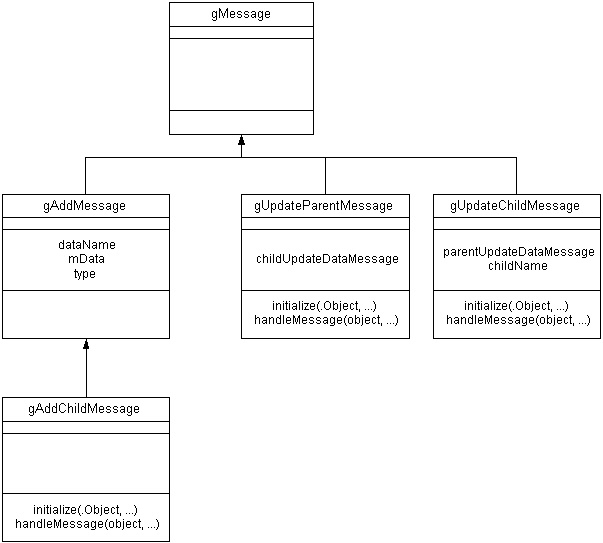
\includegraphics{MessageClass2.jpg}}
    \caption{ Inheritance for Message Classes that are Passed Between MVCs. }
    \label{Fig:BetwMess}
  \end{center}
\end{figure}

The first message class that will be discussed is \Robject{gAddChildMessage}.
A \Robject{gAddChildMessage} object will be very similar to a
\Robject{gAddDataMessage} object because they are both adding a new
model and a new MVC object.  The difference with a \Robject{gAddChildMessage}
object is that it must fill in some extra information to tie this new MVC
object to its parent MVC object.  The \Robject{gAddChildMessage} class
inherits from the \Robject{gAddMessage} class, with the same slots of
dataName, mData, and type.  The dataName slot is the name of the new model (and
new MVC), the mData slot is a list that contains the model data and virtual
data to fill the modelData and virtualData slots, respectively, of the new
model, and the type slot gives the type of the model (currently, the options
are ``exprSet'', ``graph'', or ``data.frame'').  As with the previous message
classes, the \Robject{gAddChildMessage} class has two methods:
\Rfunction{initialize} and \Rfunction{handleMessage}.  The
\Rfunction{initialize} method properly fills the slots of the object when it
is created and the \Rfunction{handleMessage} method ensures that the new model
and MVC objects are created (which is what the \Rfunction{handleMessage}
method for the \Robject{gAddDataMessage} class does) and then it fills the
linkData slot of the new child model so that the \Rfunction{linkToParent} and
\Rfunction{linkToChild} functions are available for messaging between MVC
objects and finally it stores information in the child MVC object's controller
that determines if the child model was created from a subset of the parent
model.  Thus, the \Rfunction{handleMessage} method both creates the child MVC
object and relates it to the parent MVC object.

The next two message classes pertain to updating MVC objects when a parent MVC
or child MVC object has changed.  These classes are
\Robject{gUpdateParentMessage} and \Robject{gUpdateChildMessage} and they both
inherit from the \Robject{gMessage} class, as shown in Figure
\ref{Fig:BetwMess}.  Even though they are both update messages, they do not
inherit from the \Robject{gUpdateMessage} class because the information they
need to contain is a \Robject{gUpdateDataMessage} object.  Thus, the
\Robject{gUpdateParentMessage} class has one slot, childUpdateDataMessage, and
this slot contains the \Robject{gUpdateDataMessage} object that was used to
update the child model.  Similarly, the \Robject{gUpdateChildMessage} class
has two slots, parentUpdateDataMessage and childName, where the
parentUpdateDataMessage slot contains the \Robject{gUpdateDataMessage} object
that was used to update the parent model and the childName slot contains the
name of the child model that is being updated (because a parent MVC can have
more than one child MVC). 

As with all the other message classes, these two update messages have two
methods: \Rfunction{initialize} and \Rfunction{handleMessage}.  The
\Rfunction{initialize} method properly sets the slots of the new object.  The
\Rfunction{handleMessage} method for a \Robject{gUpdateParentMessage} will
take the \Robject{gUpdateDataMessage} object from the child model and convert
it to a \Robject{gUpdateDataMessage} object for the parent model using the
\Rfunction{linkToParent} function.  Similarly, the \Rfunction{handleMessage}
method for a \Robject{gUpdateChildMessage} will take the
\Robject{gUpdateDataMessage} object from the parent model and convert it to a
\Robject{gUpdateDataMessage} object for the child model using the
\Rfunction{linkToChild} function.  

These message classes ensure that when a model is updated, its parent and
child models will be notified of the change and most importantly will be
notified of the change in a way that each model can properly act upon that
information.  Because each MVC object has a different model (and thus a
different data set and potentially a different data structure), information
that pertains to the model for one MVC must be converted to useful information
for the linked model and this conversion is done by the
\Rfunction{linkToParent} and \Rfunction{linkToChild} functions.   

\begin{figure}[ht]
  \begin{center}
    \scalebox{0.6}{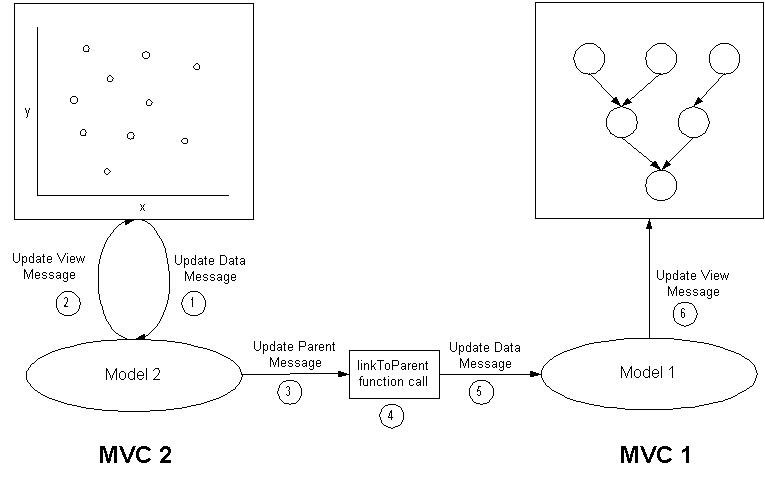
\includegraphics{MessagePassing.jpg}}
    \caption{ Message Passing Between MVCs. }
    \label{Fig:MessPass}
  \end{center}
\end{figure}

Figure \ref{Fig:MessPass} shows how messages are passed within one MVC as well
as how this message gets passed on to its parent MVC.  In this picture, the
message passing starts when a user interacts with the y vs. x scatterplot
depicting model 2.  After the user interaction with the scatterplot, step 1
(indicated on the figure as a circled 1) is to send an update data message to
model 2.  As soon as model 2 is updated, step 2 is to send an update view
message so that the scatterplot view is updated to reflect the changed data.
In step 3, an update parent message is sent because MVC 2 (which is the MVC
object for model 2) has a parent MVC, which is MVC 1.  For step 4, the
\Rfunction{linkToParent} function converts the child's update data message
into an update data message that the parent will understand.  In step 5, this
new update data message that was created by the \Rfunction{linkToParent}
function will be sent to model 1.  Finally for step 6, after model 1 has been
updated, an update view message will be sent to the view of model 1.  Now all
of the data and the views are in synch.

\section{Conclusions}\label{Sec:Conc}

Several examples of linked data sets were given at the beginning of this
paper, including linked tables from a relational database, and meta data that
is linked to experimental data.  Until now it has not been possible to create
linked views of these data sets.  However, creating linked, interactive views
of underlying linked data sets would be very helpful for exploratory data
analysis.  Thus, this paper discussed the creation of two R packages,
\Rpackage{MVCClass} and \Rpackage{iSNetwork}, which allow users to create
linked, interactive views of linked data sets based on expanding the
model-view-controller paradigm.  Now for visualizing linked data sets, the
model-view-controller design, which is a well known and thus, well tested
software paradigm, was extended to multiple MVC objects where each MVC object
contains one data set and its views.  This solution broke down the problem of
linked, interactive views of linked data sets into components (MVC objects)
that can be reused and linked.  

Although one of the goals of the \Rpackage{MVCClass} and
\Rpackage{iSNetwork} packages was to create a design that was extensible,
certain design decisions, such as expecting the data sets to be linked through
a parent-child hierarchy, may not work with some data sets.  As an example,
the linked tables from a relational database are not related through a tree
structure and thus, having parent and child MVC objects may not make sense
with these data sets.  However, the design allows users to add new
types of models, new types of views, new menu items on the control window and
new message classes so there is still flexibility for additions as long as the
data sets are connected through parent-child relationships. 

\subsection{Future Work}\label{Ssec:Further}

When a MVC's model is updated, it notifies its parent and child
MVCs that a change has occurred.  Then when a MVC gets a message from a
parent or child MVC, the MVC can either decide to ignore the message or read
the message (which results in this MVC's model being updated).  However, the
MVC object can not decide to only see certain types of messages.  It must
either accept all messages or ignore all messages.  A future goal for message
passing is to allow more selectivity in which messages will be accepted
between MVC objects so that the linking between MVC objects is more
sophisticated. 

\end{document}